%Research Plan - 20%
\section{Research Plan} 
\label{sec:research}

Given the ever-growing flood of information, Cartography provide an visually appealing way to present the world reality. The approach of this project is to visualize covid cases among different states of Northern America on the basis of per capita using cartographic mapping. 
The visualization of the covid pandemic can be classified as two types, static visualization \cite{WaPo} and complex interactive visualization \cite{CovViz} which gives overall perspective but hinder to provide details required for the user  to go in deep for the particular region and how the region is affected. This project aims to include interactive visualization and provide details of each region in the northern America on the basis of proportional statistics ie; there will be clear distinction between the severity or improvement in cases based on universal scaling and on the other hand calculating the number of cases based on total number of people in the region. 
According to work presented by Zhou et al. \cite{Zhou}, they categorize “visualization technique” as low level operation and “visual task” as interface between the visual representation and visual techniques without specifying “how” an operation is done. This project aims to facilitate both these categorization by implementing cartography based on two components such as population of each state and different metrics of covid cases in each state. In order to show the metrics such as positive cases, negative cases, total tests, recovery cases and number of death from covid in each state, we have included the mouse hover effect interaction through which, by hovering over the states, we can show details of all the metrics of the respective state. Sequential color scheme has been implemented to forecast the impact of covid and changes as per naïve data and per capita data for each metric. This project is implemented using interactive visualization for mouseover, click, mouseout and button based interactions.

\begin{figure}[h]
 \centering % avoid the use of \begin{center}...\end{center} and use \centering instead (more compact)
 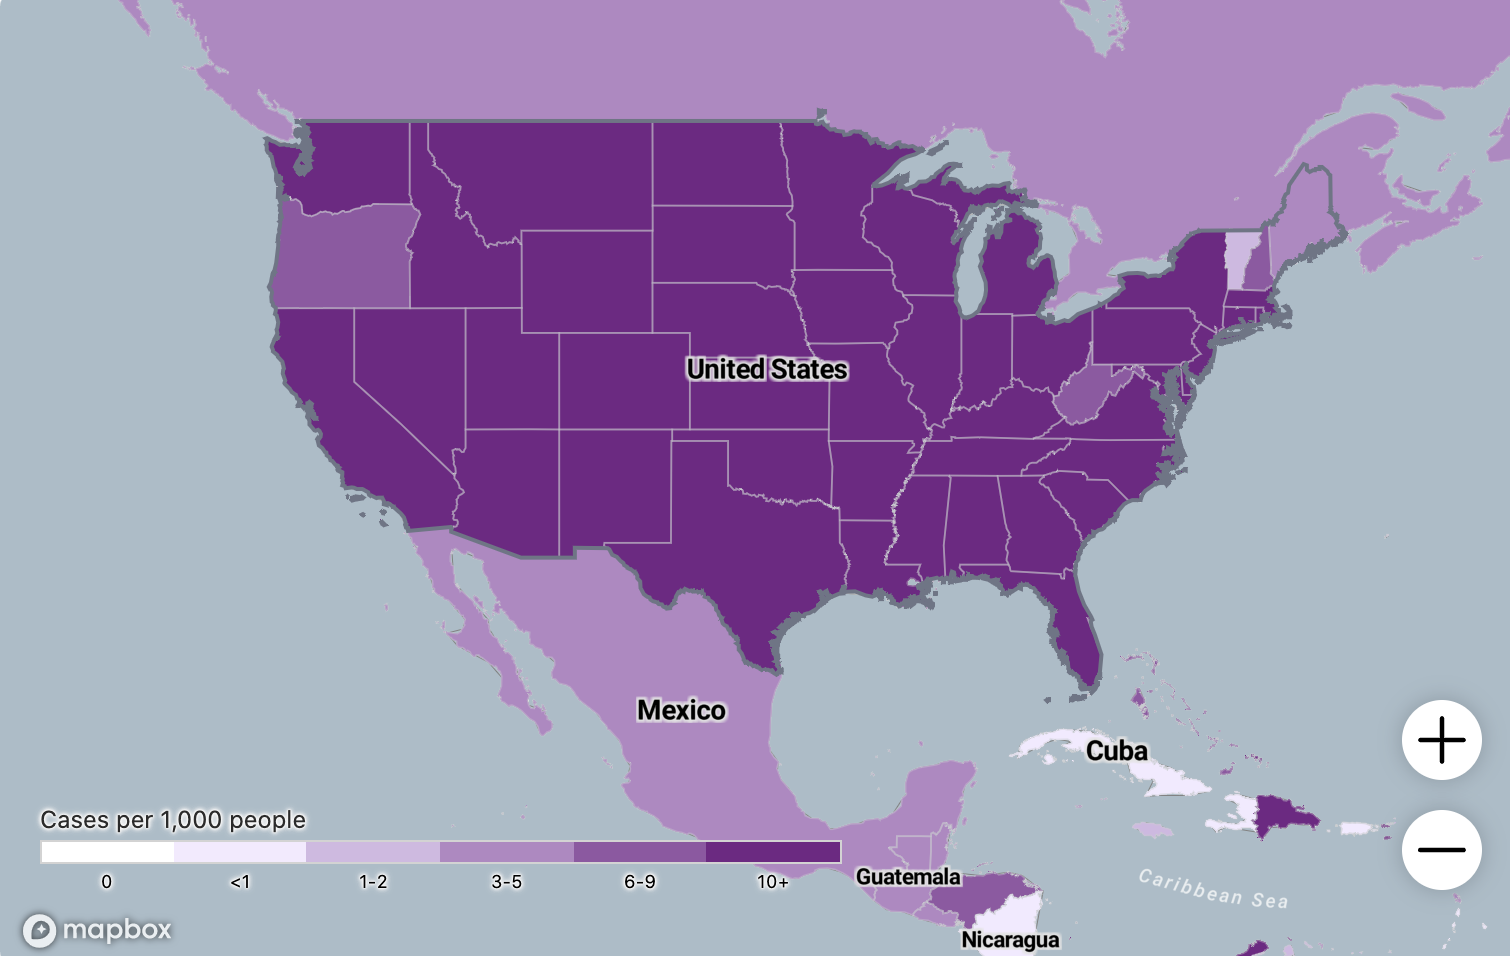
\includegraphics[width=3in]{figs/Weatherdata.png}
 \caption{Choropleth map for weather data \cite{Weather}}
 \label{fig:weather}
\end{figure}

\subsection{Data}
\label{sec:data}

Data for this project is taken from the COVID Tracking Project \cite{CTP}. This dataset includes the latest Covid-19 statistics from March till date and is updated daily. The data is categorized state-wise and shows different parameters including number of positive cases, number of negative cases etc. Population data of USA has been taken from a reference lookup table \cite{PopData}. This dataset includes total population of the country and categorized from highest to lowest as per state according to the population. 

\subsection{Evaluation}
\label{sec:eval}

The project can be evaluated on the basis of the milestones as shown in the timeline section. Some metrics for evaluation can be – efficacy of the cartographic mapping technique in showing the covid spread, the correlation plots between different categories and the implementation of additional features like mousein, mouseout, zoom etc.
Another metric is to evaluate the flexibility of the implemented visualization technique to handle changes in data since the data can change quite quickly. The visualization technique has to ensure that overcrowding doesn’t happen due to the saturation of datapoints and this becomes a key metric to ensure the data is well presented.

\subsection{Technology}
\label{sec:tech}

As D3 \cite{d3js} supports web mapping and interaction and also supports topology projection. This project will be implemented using d3.js and HTML5 and Using Topojson library \cite{top} to encode the topology. 
Above mentioned list of technologies are extremely powerful when it comes for handling geographical information. 



